\documentclass[../main.tex]{subfiles}
\begin{document}
%=========================================================
% TĐ_PBT_PRE1_HK1_Tuan18
% Phiếu bài tập PRE1 - Tuần 18
%   Toán: Luyện tập chung - Ôn tập kiểm tra (trọng tâm: phép trừ trong phạm vi 6)
% Soạn theo mẫu (\hktuan, bt, listEX)
% Toàn bộ hình vẽ bằng TikZ (không cần thư mục hình), tông màu pastel
% Tiền tố lệnh riêng: PH (hình/màu), TT (lệnh dùng chung với các phiếu khác)
%=========================================================

%---------- Lệnh dùng chung cho phiếu ----------
\providecommand{\TTcham}[1][3cm]{\makebox[#1]{\dotfill}}
\providecommand{\TTthongtin}{%
  \noindent\begin{tabular}{|p{7.6cm}|p{4cm}|p{4cm}|}
    \hline
    \textbf{Họ và Tên HS:}\dotfill & \textbf{Lớp:}\dotfill & \textbf{Ngày:}\dotfill \\
    \hline
  \end{tabular}\par\medskip}
\makeatletter
\providecommand{\TTdatlaibai}{\@ifundefined{c@bt}{}{\setcounter{bt}{0}}}
\makeatother
\providecommand{\TTbatdauhinh}{}\renewcommand{\TTbatdauhinh}{\par\nopagebreak\vspace{4pt}\nopagebreak}

\usetikzlibrary{arrows.meta,shapes.geometric,calc,positioning}

%---------- Bảng màu pastel ----------
\definecolor{PHdo}{RGB}{240,128,134}\definecolor{PHdodam}{RGB}{196,82,92}
\definecolor{PHxanh}{RGB}{150,208,158}\definecolor{PHxanhdam}{RGB}{82,156,108}
\definecolor{PHbien}{RGB}{156,204,240}\definecolor{PHbiendam}{RGB}{86,146,206}
\definecolor{PHvang}{RGB}{255,230,150}\definecolor{PHvangdam}{RGB}{232,184,76}
\definecolor{PHhong}{RGB}{250,190,208}\definecolor{PHcam}{RGB}{255,200,146}
\definecolor{PHnau}{RGB}{196,146,112}\definecolor{PHnaudam}{RGB}{142,96,70}
\definecolor{PHtim}{RGB}{208,192,238}\definecolor{PHda}{RGB}{255,226,200}
\definecolor{PHnen}{RGB}{255,249,232}\definecolor{PHkhung}{RGB}{136,158,206}
\definecolor{PHmint}{RGB}{190,232,214}\definecolor{PHxam}{RGB}{120,128,150}

\tikzset{
  PHo/.style={draw=PHkhung!90!black,thick,rounded corners=3pt,fill=white,minimum size=0.9cm,inner sep=0pt,font=\sffamily\bfseries\Large},
  PHotron/.style={draw=PHkhung!90!black,thick,circle,fill=white,minimum size=0.95cm,inner sep=0pt,font=\sffamily\bfseries\Large},
}

%=========================================================
%        THƯ VIỆN HÌNH NHỎ (vẽ tại gốc tọa độ, cao khoảng 0,8 cm)
%=========================================================
% Cây thông Giáng sinh
\providecommand{\PHcay}{}\renewcommand{\PHcay}{%
  \begin{scope}[line join=round]
  \fill[PHnau,draw=PHnaudam,thin,rounded corners=1pt] (-0.06,-0.43) rectangle (0.06,-0.26);
  \foreach \y/\w in {-0.3/0.33,-0.1/0.27,0.08/0.21}{%
    \path[top color=PHxanh!90!white,bottom color=PHxanhdam!85!PHxanh,draw=PHxanhdam!85!black,thin,rounded corners=1.8pt]
      (-\w,\y) -- (0,\y+0.34) -- (\w,\y) -- cycle;}
  \node[star,star points=5,star point ratio=2.1,fill=PHvang,draw=PHvangdam,thin,inner sep=0pt,minimum size=0.17cm] at (0,0.43) {};
  \fill[PHdo] (-0.1,-0.2) circle (0.032); \fill[PHvang] (0.12,-0.14) circle (0.032);
  \fill[PHbien] (0,-0.02) circle (0.03); \fill[PHdo] (-0.06,0.12) circle (0.028);
  \fill[PHvang] (0.07,0.2) circle (0.026);
  \end{scope}}
% Hộp quà (tham số: màu hộp)
\providecommand{\PHqua}{}\renewcommand{\PHqua}[1]{%
  \shade[top color=#1!55!white,bottom color=#1,draw=#1!60!black,thin,rounded corners=1.5pt] (-0.29,-0.32) rectangle (0.29,0.12);
  \shade[top color=#1!40!white,bottom color=#1!90!white,draw=#1!60!black,thin,rounded corners=1.5pt] (-0.34,0.08) rectangle (0.34,0.24);
  \fill[PHvang!90!PHvangdam] (-0.055,-0.32) rectangle (0.055,0.24);
  \foreach \s in {1,-1}{\begin{scope}[xscale=\s]
    \fill[PHvang,draw=PHvangdam,thin] (0,0.26) .. controls (-0.04,0.42) and (-0.26,0.46) .. (-0.24,0.33) .. controls (-0.22,0.25) and (-0.08,0.25) .. (0,0.26);
  \end{scope}}
  \fill[PHvangdam] (0,0.26) circle (0.04);}
% Kẹo mút
\providecommand{\PHkeo}{}\renewcommand{\PHkeo}{%
  \draw[PHnau!70!white,line width=2.2pt,line cap=round] (0,-0.1) -- (0,-0.42);
  \fill[white] (0,0.14) circle (0.27);
  \foreach \a in {0,60,...,300}{\fill[PHdo!85!white] (0,0.14) -- ++(\a:0.27) arc (\a:\a+32:0.27) -- cycle;}
  \draw[PHdo,thin] (0,0.14) circle (0.27);
  \fill[white,opacity=0.55] (-0.13,0.27) ellipse (0.045 and 0.08);
  \fill[PHxanh,draw=PHxanhdam,thin] (0,-0.13) -- (-0.1,-0.07) -- (-0.1,-0.19) -- cycle;
  \fill[PHxanh,draw=PHxanhdam,thin] (0,-0.13) -- (0.1,-0.07) -- (0.1,-0.19) -- cycle;
  \fill[PHxanhdam] (0,-0.13) circle (0.025);}
% Bánh quy hình người
\providecommand{\PHbanh}{}\renewcommand{\PHbanh}{%
  \begin{scope}[line join=round,line cap=round]
  \def\PHbanhhinh{(-0.36,0.12) -- (-0.17,0.17) -- (0.17,0.17) -- (0.36,0.12) -- (0.39,-0.01) -- (0.18,-0.03) -- (0.2,-0.39) -- (0.04,-0.39) -- (0,-0.17) -- (-0.04,-0.39) -- (-0.2,-0.39) -- (-0.18,-0.03) -- (-0.39,-0.01) -- cycle}
  \draw[PHnaudam!80,line width=1.5pt,rounded corners=2.5pt] \PHbanhhinh;
  \draw[PHnaudam!80,line width=1.5pt] (0,0.3) circle (0.14);
  \fill[PHcam!95!PHnau,rounded corners=2.5pt] \PHbanhhinh;
  \fill[PHcam!95!PHnau] (0,0.3) circle (0.14);
  \draw[white,line width=0.9pt] (-0.35,0.06) -- (-0.22,0.09) (0.35,0.06) -- (0.22,0.09) (-0.18,-0.3) -- (-0.07,-0.3) (0.18,-0.3) -- (0.07,-0.3);
  \fill[PHnaudam] (-0.05,0.33) circle (0.02) (0.05,0.33) circle (0.02);
  \draw[PHnaudam,thin] (-0.05,0.26) arc (200:340:0.055);
  \fill[PHhong!80,opacity=0.8] (-0.09,0.27) circle (0.025) (0.09,0.27) circle (0.025);
  \fill[PHdo] (0,0.08) circle (0.03) (0,-0.02) circle (0.03);
  \end{scope}}
% Người tuyết
\providecommand{\PHtuyet}{}\renewcommand{\PHtuyet}{%
  \draw[PHnaudam,line width=1.1pt,line cap=round] (-0.2,-0.1) -- (-0.4,0.0) (-0.33,-0.04) -- (-0.4,-0.1) (0.2,-0.1) -- (0.4,0.02) (0.33,-0.03) -- (0.4,0.1);
  \shade[inner color=white,outer color=PHbien!45!white,draw=PHbiendam!70,thin] (0,-0.17) circle (0.25);
  \shade[inner color=white,outer color=PHbien!45!white,draw=PHbiendam!70,thin] (0,0.17) circle (0.16);
  \fill[PHxanhdam!85,rounded corners=1pt] (-0.19,0.3) rectangle (0.19,0.33);
  \fill[PHxanh!85!PHxanhdam,draw=PHxanhdam,thin,rounded corners=1.2pt] (-0.11,0.325) rectangle (0.11,0.47);
  \fill[PHdo] (-0.11,0.325) rectangle (0.11,0.365);
  \fill[PHnaudam] (-0.05,0.2) circle (0.02) (0.05,0.2) circle (0.02);
  \fill[PHcam,draw=PHnau,very thin] (0.0,0.16) -- (0.17,0.13) -- (0.0,0.12) -- cycle;
  \fill[PHdo,rounded corners=1.5pt] (-0.17,0.0) rectangle (0.17,0.07);
  \fill[PHdo] (0.07,0.0) -- (0.16,0.0) -- (0.17,-0.17) -- (0.09,-0.16) -- cycle;
  \fill[PHnaudam] (0,-0.1) circle (0.025) (0,-0.2) circle (0.025) (0,-0.3) circle (0.025);}
% Quả châu (tham số: màu)
\providecommand{\PHchuong}{}\renewcommand{\PHchuong}[1]{%
  \shade[inner color=#1!30!white,outer color=#1,draw=#1!65!black,thin] (0,-0.1) circle (0.27);
  \draw[white,line width=1.2pt,opacity=0.9,line join=round] (-0.26,-0.12) -- (-0.17,-0.05) -- (-0.08,-0.12) -- (0.01,-0.05) -- (0.1,-0.12) -- (0.19,-0.05) -- (0.26,-0.12);
  \fill[PHvang,draw=PHvangdam,thin] (-0.07,0.15) rectangle (0.07,0.24);
  \draw[PHvangdam,thick] (0,0.24) circle (0.045);
  \fill[white,opacity=0.55] (-0.12,0.03) ellipse (0.045 and 0.09);}
% Chiếc tất
\providecommand{\PHtat}{}\renewcommand{\PHtat}{%
  \shade[top color=PHdo!85!white,bottom color=PHdo,draw=PHdodam,thin,rounded corners=1pt]
    (-0.15,0.3) -- (0.17,0.3) -- (0.17,-0.05) .. controls (0.2,-0.14) and (0.42,-0.1) .. (0.42,-0.27) .. controls (0.42,-0.42) and (-0.06,-0.42) .. (-0.13,-0.25) -- cycle;
  \fill[white,draw=PHxam!50,thin,rounded corners=2pt] (-0.19,0.22) rectangle (0.21,0.4);
  \fill[PHvang] (0.2,-0.3) .. controls (0.3,-0.4) and (0.4,-0.38) .. (0.41,-0.28) .. controls (0.35,-0.3) .. (0.2,-0.3);
  \fill[PHvang] (-0.12,-0.28) .. controls (-0.08,-0.4) .. (0.0,-0.38) .. controls (-0.04,-0.33) .. (-0.12,-0.28);
  \fill[white,opacity=0.8] (-0.05,0.08) circle (0.025) (0.06,0.0) circle (0.025) (-0.02,-0.1) circle (0.025);}
% Mũ ông già Noel
\providecommand{\PHnon}{}\renewcommand{\PHnon}{%
  \shade[top color=PHdo!85!white,bottom color=PHdo,draw=PHdodam,thin]
    (-0.36,-0.12) .. controls (-0.3,0.2) and (0.0,0.3) .. (0.3,0.14) .. controls (0.36,0.06) and (0.38,-0.02) .. (0.36,-0.12) -- cycle;
  \fill[white,draw=PHxam!40,thin,rounded corners=4pt] (-0.42,-0.27) rectangle (0.42,-0.08);
  \foreach \x in {-0.3,-0.1,0.1,0.3}{\fill[white] (\x,-0.27) circle (0.04);}
  \fill[white,draw=PHxam!40,thin] (0.31,0.18) circle (0.075);}
% Quả táo
\providecommand{\PHtao}{}\renewcommand{\PHtao}{%
  \shade[inner color=PHdo!40!white,outer color=PHdo,draw=PHdodam,thin]
    (0,0.2) .. controls (-0.12,0.32) and (-0.4,0.28) .. (-0.38,-0.05) .. controls (-0.36,-0.3) and (-0.16,-0.4) .. (0,-0.3) .. controls (0.16,-0.4) and (0.36,-0.3) .. (0.38,-0.05) .. controls (0.4,0.28) and (0.12,0.32) .. (0,0.2);
  \draw[PHnaudam,thick,line cap=round] (0,0.2) -- (0.03,0.38);
  \fill[PHxanh,draw=PHxanhdam,thin] (0.03,0.34) .. controls (0.1,0.5) and (0.26,0.46) .. (0.28,0.38) .. controls (0.2,0.28) and (0.09,0.3) .. (0.03,0.34);
  \fill[white,opacity=0.55] (-0.2,0.1) ellipse (0.045 and 0.09);}
% Quả dâu tây
\providecommand{\PHdau}{}\renewcommand{\PHdau}{%
  \shade[inner color=PHdo!45!white,outer color=PHdo,draw=PHdodam,thin] (0,-0.38) .. controls (-0.3,-0.2) and (-0.38,0.08) .. (-0.2,0.22) .. controls (-0.08,0.28) and (0.08,0.28) .. (0.2,0.22) .. controls (0.38,0.08) and (0.3,-0.2) .. (0,-0.38);
  \foreach \x/\y in {-0.14/0.1,0/0.13,0.14/0.1,-0.19/-0.03,-0.07/-0.01,0.07/-0.01,0.19/-0.03,-0.11/-0.15,0.02/-0.14,0.12/-0.15,0.0/-0.27}{\fill[PHvang] (\x,\y) ellipse (0.015 and 0.025);}
  \fill[PHxanh,draw=PHxanhdam,thin] (0,0.24) -- (-0.17,0.3) -- (-0.07,0.33) -- (-0.1,0.4) -- (0,0.35) -- (0.1,0.4) -- (0.07,0.33) -- (0.17,0.3) -- cycle;}
% Ông già Noel (đầu) - cao khoảng 1,5 cm
\providecommand{\PHongla}{}\renewcommand{\PHongla}{%
  \begin{scope}[line join=round]
  \shade[top color=PHdo!85!white,bottom color=PHdo,draw=PHdodam,thin] (-0.5,0.3) .. controls (-0.5,0.8) and (0.0,1.0) .. (0.52,0.62) .. controls (0.35,0.55) and (0.3,0.4) .. (0.5,0.28) -- cycle;
  \fill[white,draw=PHxam!40,thin] (0.55,0.68) circle (0.14);
  \fill[white,draw=PHxam!65,thin] (-0.45,0.0) .. controls (-0.7,-0.5) and (-0.35,-0.95) .. (0,-0.95) .. controls (0.35,-0.95) and (0.7,-0.5) .. (0.45,0.0) -- cycle;
  \fill[PHda,draw=PHnau,thin] (0,0.0) ellipse (0.38 and 0.34);
  \fill[white,draw=PHxam!40,thin,rounded corners=6pt] (-0.5,0.2) rectangle (0.5,0.42);
  \foreach \x in {-0.38,-0.19,0,0.19,0.38}{\fill[white] (\x,0.2) circle (0.075);}
  \fill[white,draw=PHxam!40,thin] (-0.02,-0.3) .. controls (-0.3,-0.12) and (-0.4,-0.38) .. (-0.18,-0.5) .. controls (0,-0.42) and (0.0,-0.3) .. (-0.02,-0.3);
  \fill[white,draw=PHxam!40,thin] (0.02,-0.3) .. controls (0.3,-0.12) and (0.4,-0.38) .. (0.18,-0.5) .. controls (0,-0.42) and (0,-0.3) .. (0.02,-0.3);
  \fill[PHhong] (0,-0.08) circle (0.065);
  \fill[PHhong!80,opacity=0.7] (-0.24,-0.08) circle (0.07) (0.24,-0.08) circle (0.07);
  \fill[PHnaudam] (-0.14,0.07) circle (0.025) (0.14,0.07) circle (0.025);
  \draw[PHnaudam,thin,line cap=round] (-0.04,-0.3) arc (200:340:0.045);
  \end{scope}}
% Bàn tay giơ n ngón (n = 0..5): ngón trỏ, giữa, áp út, út rồi đến ngón cái
\providecommand{\PHtay}{}\renewcommand{\PHtay}[1]{%
  \begin{scope}[line join=round,line cap=round]
  \def\PHtayda{PHda}\def\PHtayvien{PHnau}
  \foreach \x/\h/\id in {-0.2/0.5/1,-0.07/0.56/2,0.06/0.52/3,0.19/0.42/4}{%
    \ifnum#1<\id
      \filldraw[fill=\PHtayda,draw=\PHtayvien,thick,rounded corners=3pt] (\x-0.055,-0.02) rectangle (\x+0.055,0.12);
    \else
      \filldraw[fill=\PHtayda,draw=\PHtayvien,thick,rounded corners=3pt] (\x-0.055,-0.02) rectangle (\x+0.055,\h);
      \draw[\PHtayvien!70,thin] (\x-0.03,\h*0.45) -- (\x+0.03,\h*0.45);
    \fi}
  \ifnum#1>4
    \filldraw[fill=\PHtayda,draw=\PHtayvien,thick,rounded corners=3pt,rotate around={32:(-0.3,-0.2)}] (-0.36,-0.2) rectangle (-0.24,0.28);
  \else
    \filldraw[fill=\PHtayda,draw=\PHtayvien,thick,rounded corners=3pt,rotate around={-20:(-0.3,-0.2)}] (-0.38,-0.22) rectangle (-0.22,-0.02);
  \fi
  \filldraw[fill=\PHtayda,draw=\PHtayvien,thick,rounded corners=6pt] (-0.3,-0.48) rectangle (0.3,0.03);
  \foreach \x in {-0.2,-0.07,0.06,0.19}{\fill[\PHtayda] (\x-0.05,-0.01) rectangle (\x+0.05,0.05);}
  \end{scope}}
% Bé gấu
\providecommand{\PHgau}{}\renewcommand{\PHgau}{%
  \foreach \s in {1,-1}{\begin{scope}[xscale=\s]\fill[PHnau,draw=PHnaudam,thin] (0.3,0.3) circle (0.15);\fill[PHcam!70] (0.3,0.3) circle (0.08);\end{scope}}
  \shade[inner color=PHnau!70!white,outer color=PHnau,draw=PHnaudam,thin] (0,0) circle (0.42);
  \fill[PHda,draw=PHnau!80,thin] (0,-0.11) ellipse (0.19 and 0.15);
  \fill[PHnaudam] (0,-0.03) ellipse (0.055 and 0.04);
  \fill[PHnaudam] (-0.15,0.1) circle (0.03) (0.15,0.1) circle (0.03);
  \draw[PHnaudam,thin,line cap=round] (0,-0.07) -- (0,-0.12) (-0.07,-0.16) arc (200:340:0.07);}
% Chồng bánh kếp có xi-rô (rộng khoảng 0,9 cm)
\providecommand{\PHbanhkep}{}\renewcommand{\PHbanhkep}{%
  \fill[PHbien!40!white,draw=PHxam!35,thin] (0,-0.27) ellipse (0.46 and 0.12);
  \foreach \j in {0,1,2}{%
    \fill[PHcam!90!PHnau,draw=PHnau,thin] (-0.3,-0.22+0.1*\j) -- (-0.3,-0.14+0.1*\j) arc (180:360:0.3 and 0.07) -- (0.3,-0.22+0.1*\j) arc (0:-180:0.3 and 0.07) -- cycle;}
  \fill[PHcam!70!white,draw=PHnau,thin] (0,0.0) ellipse (0.3 and 0.075);
  \fill[PHnaudam!85!PHnau] (-0.2,0.0) .. controls (-0.2,0.05) and (0.2,0.05) .. (0.2,0.0) .. controls (0.22,-0.08) and (0.14,-0.12) .. (0.13,-0.04) .. controls (0.1,-0.1) and (0.02,-0.14) .. (0.0,-0.04) .. controls (-0.04,-0.14) and (-0.12,-0.12) .. (-0.12,-0.04) .. controls (-0.14,-0.1) and (-0.2,-0.08) .. (-0.2,0.0);
  \fill[PHvang,draw=PHvangdam,thin,rounded corners=0.5pt] (-0.05,-0.01) rectangle (0.07,0.07);}
% Gạch chéo một hình
\providecommand{\PHgach}{}\renewcommand{\PHgach}{\draw[PHdodam,line width=1.7pt,line cap=round,opacity=0.85] (-0.38,-0.4) -- (0.38,0.42);}

%=========================================================
%        BỐ CỤC CHUNG
%=========================================================
% Khoảng cách giữa các hàng hình
\providecommand{\PHcach}{}\renewcommand{\PHcach}{\par\vspace{5pt}}

% Hàng vật thể (n vật, k vật cuối bị gạch); nằm trong tikzpicture: \PHday{vật}{n}{k}
\providecommand{\PHday}{}\renewcommand{\PHday}[3]{%
  \pgfmathtruncatemacro{\PHgiu}{#2-#3}%
  \foreach \i in {1,...,#2}{%
    \begin{scope}[shift={(1.1*\i-1.1,0)},scale=1.25]#1\ifnum\i>\PHgiu\PHgach\fi\end{scope}}}
% Dấu và ô: \PHbieuthuc{x}{y}{a}{dấu}{b}{c} đặt biểu thức a dấu b = c với a tại x,y
\providecommand{\PHbieuthuc}{}\renewcommand{\PHbieuthuc}[6]{%
  \node[PHo] at (#1,#2) {#3};
  \node[font=\sffamily\bfseries\LARGE] at (#1+0.8,#2) {#4};
  \node[PHo] at (#1+1.6,#2) {#5};
  \node[font=\sffamily\bfseries\LARGE] at (#1+2.4,#2) {$=$};
  \node[PHo] at (#1+3.2,#2) {#6};}
% Phép tính đứng riêng: \PHpt{a}{dấu}{b}{c}
\providecommand{\PHpt}{}\renewcommand{\PHpt}[4]{%
  \begin{tikzpicture}[font=\sffamily\Large]\PHbieuthuc{0}{0}{#1}{#2}{#3}{#4}\end{tikzpicture}}
% Khung nền cho một hàng: \PHkhung{rộng}{cao}
\providecommand{\PHkhung}{}\renewcommand{\PHkhung}[2]{%
  \draw[PHkhung,thick,rounded corners=10pt,fill=PHnen] (-0.5,-#2/2) rectangle (#1-0.5,#2/2);}
% Một hàng phép tính bằng tranh (đã/ chưa gạch): vật, n, k gạch, a, b, c  (để trống = HS điền)
\providecommand{\PHphep}{}\renewcommand{\PHphep}[6]{%
  \begin{tikzpicture}[font=\sffamily\Large]
    \PHkhung{15.6}{1.5}
    \begin{scope}[shift={(0.4,0)}]\PHday{#1}{#2}{#3}\end{scope}
    \PHbieuthuc{10.6}{0}{#4}{$-$}{#5}{#6}
  \end{tikzpicture}\par}
% Hàng phép cộng bằng tranh: vật 1, a, vật 2, b, kết quả
\providecommand{\PHcongday}{}\renewcommand{\PHcongday}[5]{%
  \begin{tikzpicture}[font=\sffamily\Large]
    \PHkhung{15.6}{1.5}
    \begin{scope}[shift={(0.4,0)}]\PHday{#1}{#2}{0}\end{scope}
    \node[font=\sffamily\bfseries\LARGE] at (1.1*#2+0.3,0) {$+$};
    \begin{scope}[shift={(1.1*#2+1.2,0)}]\PHday{#3}{#4}{0}\end{scope}
    \node[font=\sffamily\bfseries\LARGE] at (12.9,0) {$=$};
    \node[PHo] at (13.9,0) {#5};
  \end{tikzpicture}\par}

%---------- Rải vật thể tự nhiên trong một ô đếm ----------
\def\PHviA{0/0}\def\PHviB{0/0}
\def\PHviC{-0.8/0.1,0.8/-0.05}
\def\PHviD{-1.3/0.15,0/-0.15,1.3/0.2}
\def\PHviE{-1.5/0.15,-0.5/-0.2,0.5/0.2,1.5/-0.1}
\def\PHviF{-1.7/0.1,-0.85/-0.2,0/0.22,0.85/-0.15,1.7/0.15}
\def\PHviG{-1.95/0.2,-1.15/-0.22,-0.35/0.24,0.4/-0.18,1.15/0.22,1.95/-0.1}
\providecommand{\PHrai}{}\renewcommand{\PHrai}[2]{% vật, số lượng (2..6)
  \expandafter\let\expandafter\PHdsvt\csname PHvi\ifcase#2 A\or A\or C\or D\or E\or F\or G\fi\endcsname
  \foreach \x/\y in \PHdsvt {\begin{scope}[shift={(\x,\y+0.12)},scale=1.45]#1\end{scope}}}
% Một ô đếm: \PHodem{vật}{số lượng}{đáp án (hiện cho mẫu)}
\providecommand{\PHodem}{}\renewcommand{\PHodem}[3]{%
  \begin{tikzpicture}[font=\sffamily\Large]
    \draw[PHkhung,thick,rounded corners=12pt,fill=PHnen] (-2.55,-1.3) rectangle (2.55,1.2);
    \PHrai{#1}{#2}
    \node[PHo,minimum width=1.5cm,minimum height=0.85cm,rounded corners=10pt] at (0,-1.3) {\textcolor{PHdodam}{#3}};
  \end{tikzpicture}}

%---------- Ô táo chứa kết quả ----------
\providecommand{\PHodtao}{}\renewcommand{\PHodtao}[1]{%
  \begin{tikzpicture}[font=\sffamily\bfseries\Large]
    \node[anchor=east] at (0,0) {#1\ $=$};
    \begin{scope}[shift={(0.8,0)},scale=1.9]
      \shade[inner color=PHdo!12!white,outer color=PHdo!35!white,draw=PHdodam!70,thick]
        (0,0.2) .. controls (-0.12,0.32) and (-0.4,0.28) .. (-0.38,-0.05) .. controls (-0.36,-0.3) and (-0.16,-0.4) .. (0,-0.3) .. controls (0.16,-0.4) and (0.36,-0.3) .. (0.38,-0.05) .. controls (0.4,0.28) and (0.12,0.32) .. (0,0.2);
      \draw[PHnaudam,thick,line cap=round] (0,0.2) -- (0.03,0.4);
      \fill[PHxanh,draw=PHxanhdam,thin] (0.03,0.35) .. controls (0.1,0.52) and (0.26,0.48) .. (0.28,0.4) .. controls (0.2,0.3) and (0.09,0.32) .. (0.03,0.35);
    \end{scope}
  \end{tikzpicture}}

%---------- Ông già Noel cầm bảng phép tính / hộp quà có số ----------
\providecommand{\PHongnoel}{}\renewcommand{\PHongnoel}[1]{%
  \begin{scope}[scale=1.25,shift={(0,0.1)}]\PHongla\end{scope}
  \node[draw=PHkhung!90!black,thick,fill=white,rounded corners=2pt,minimum width=2.1cm,minimum height=0.8cm,font=\sffamily\bfseries\Large] at (0,-0.85) {#1};}
\providecommand{\PHhopso}{}\renewcommand{\PHhopso}[1]{%
  \begin{scope}[scale=2.3]\PHqua{PHxanh}\end{scope}
  \node[draw=PHxanhdam,thick,fill=white,rounded corners=2pt,minimum size=0.75cm,font=\sffamily\bfseries\Large] at (0,-0.12) {#1};}

%---------- Hoa hướng dương trong chậu: \PHchau{số trong chậu}{hoa trái}{hoa phải} ----------
\providecommand{\PHhoa}{}\renewcommand{\PHhoa}[3]{% tâm hoa tại gốc, bán kính nhụy 0,33
  \foreach \a in {0,30,...,330}{\fill[PHvang!95!PHvangdam,draw=PHvangdam,very thin] (\a:0.4) ellipse (0.17 and 0.1);}
  \foreach \a in {0,30,...,330}{\begin{scope}[rotate=\a]\fill[PHvang!95!PHvangdam,draw=PHvangdam,very thin] (0.37,0) ellipse (0.15 and 0.085);\end{scope}}
  \node[PHotron,minimum size=0.72cm,font=\sffamily\bfseries\large] at (0,0) {#1};}
\providecommand{\PHchau}{}\renewcommand{\PHchau}[3]{%
  \begin{tikzpicture}[font=\sffamily]
    \draw[PHxanhdam,line width=2.2pt,line cap=round] (0,0.1) .. controls (-0.2,0.6) and (-0.55,0.9) .. (-0.7,1.25);
    \draw[PHxanhdam,line width=2.2pt,line cap=round] (0,0.1) .. controls (0.2,0.5) and (0.55,0.75) .. (0.78,0.95);
    \begin{scope}[shift={(-0.75,1.45)},scale=1.0]\PHhoa{#2}{}{}\end{scope}
    \begin{scope}[shift={(0.85,1.15)},scale=0.95]\PHhoa{#3}{}{}\end{scope}
    \shade[left color=PHnau!90!white,right color=PHnau!70!PHnaudam,draw=PHnaudam,thick,rounded corners=3pt] (-0.7,-1.0) -- (0.7,-1.0) -- (0.55,0.0) -- (-0.55,0.0) -- cycle;
    \fill[PHnau!70!PHnaudam,draw=PHnaudam,thick,rounded corners=2pt] (-0.78,0.0) rectangle (0.78,0.2);
    \node[PHotron,minimum size=0.9cm] at (0,-0.5) {#1};
  \end{tikzpicture}}

%---------- Một cảnh "đã đi mất": \PHcanh{vật}{còn lại}{đã đi} ----------
\providecommand{\PHcanh}{}\renewcommand{\PHcanh}[3]{%
  \begin{tikzpicture}[font=\sffamily\Large]
    \draw[PHbien!80,thick,rounded corners=12pt,top color=PHbien!6,bottom color=PHbien!32] (-0.6,-0.85) rectangle (3.7,0.95);
    \foreach \i in {1,...,#2}{\begin{scope}[shift={(0.9*\i-0.4,0.05)},scale=1.15]#1\end{scope}}
    \draw[PHxam,thick,dashed,-{Stealth[length=2.5mm]}] (3.85,0.05) -- (4.55,0.05);
    \foreach \i in {1,...,#3}{\begin{scope}[shift={(4.5+0.72*\i,0.05)},scale=0.85]#1\end{scope}}
  \end{tikzpicture}}

%---------- Nhảy lùi trên tia số: \PHtiaso{bắt đầu}{lùi}{1 nếu vẽ sẵn các cung} ----------
\providecommand{\PHtiaso}{}\renewcommand{\PHtiaso}[3]{%
  \begin{tikzpicture}[font=\sffamily\bfseries\large]
    \draw[PHxam,very thick,-{Stealth[length=3mm]}] (-0.4,0) -- (7.7,0);
    \foreach \n in {0,...,6}{\draw[PHxam,thick] (1.1*\n,-0.1) -- (1.1*\n,0.1);\node[below=3pt] at (1.1*\n,-0.08) {\n};}
    \fill[PHdo] (1.1*#1,0.0) circle (0.12);
    \ifnum#3=1
      \foreach \j in {1,...,#2}{\draw[PHbiendam,thick,-{Stealth[length=2.5mm]}] (1.1*#1-1.1*\j+1.1,0.08) to[bend right=55] (1.1*#1-1.1*\j,0.08);}
    \fi
  \end{tikzpicture}}

%---------- Sơ đồ tách số: \PHtach{tổng}{trái}{phải} ----------
\providecommand{\PHtach}{}\renewcommand{\PHtach}[3]{%
  \begin{tikzpicture}[font=\sffamily]
    \draw[PHkhung,thick] (0,0.1) -- (-0.8,-0.85) (0,0.1) -- (0.8,-0.85);
    \node[PHotron,fill=PHvang!70] at (0,0.55) {#1};
    \node[PHotron,fill=PHbien!35] at (-0.8,-1.2) {#2};
    \node[PHotron,fill=PHhong!45] at (0.8,-1.2) {#3};
  \end{tikzpicture}}


% Hàng vật nhỏ gọn (cho ô nhỏ): \PHdaynho{vật}{n}{k gạch}
\providecommand{\PHdaynho}{}\renewcommand{\PHdaynho}[3]{%
  \pgfmathtruncatemacro{\PHgiu}{#2-#3}%
  \foreach \i in {1,...,#2}{%
    \begin{scope}[shift={(0.68*\i-0.68,0)},scale=0.8]#1\ifnum\i>\PHgiu\PHgach\fi\end{scope}}}
% Ô tròn để chọn dấu
\providecommand{\PHovong}{}\renewcommand{\PHovong}{\tikz[baseline=-0.6ex]\draw[PHkhung!90!black,thick,fill=white] (0,0) circle (0.33);}
% Hàng có tranh tự do + biểu thức chọn dấu: \PHdaukhung{mã hình}{a}{b}{c}
\providecommand{\PHdaukhung}{}\renewcommand{\PHdaukhung}[4]{%
  \begin{tikzpicture}[font=\sffamily\Large]
    \PHkhung{15.6}{1.5}
    \begin{scope}[shift={(0.4,0)}]#1\end{scope}
    \PHbieuthuc{10.6}{0}{#2}{\PHovong}{#3}{#4}
  \end{tikzpicture}\par}
% Hàng có một nhân vật dẫn chuyện + vật + phép trừ để trống: \PHphepx{nhân vật}{vật}{n}{k}
\providecommand{\PHphepx}{}\renewcommand{\PHphepx}[4]{%
  \begin{tikzpicture}[font=\sffamily\Large]
    \PHkhung{15.6}{1.5}
    \begin{scope}[shift={(0.4,0)}]#1\end{scope}
    \begin{scope}[shift={(2.4,0)}]\PHday{#2}{#3}{#4}\end{scope}
    \PHbieuthuc{10.6}{0}{}{$-$}{}{}
  \end{tikzpicture}\par}
% Hàng so sánh số lượng hình: \PHsosanh{vật trái}{n}{vật phải}{m}
\providecommand{\PHsosanh}{}\renewcommand{\PHsosanh}[4]{%
  \begin{tikzpicture}[font=\sffamily\Large]
    \PHkhung{15.6}{1.5}
    \begin{scope}[shift={(0.4,0)}]\PHday{#1}{#2}{0}\end{scope}
    \node[PHotron,minimum size=0.95cm] at (7.1,0) {};
    \begin{scope}[shift={(8.7,0)}]\PHday{#3}{#4}{0}\end{scope}
  \end{tikzpicture}\par}
% Hàng Đúng/Sai: \PHds{vật}{n}{k gạch}{phép tính}
\providecommand{\PHds}{}\renewcommand{\PHds}[4]{%
  \begin{tikzpicture}[font=\sffamily\Large]
    \PHkhung{15.6}{1.5}
    \begin{scope}[shift={(0.4,0)}]\PHday{#1}{#2}{#3}\end{scope}
    \node[font=\sffamily\bfseries\LARGE,anchor=west] at (9.2,0) {#4};
    \node[PHo,minimum size=0.95cm] at (14.1,0) {};
  \end{tikzpicture}\par}
% Ô điền số còn thiếu có hình minh họa: \PHodien{vật}{a}{dấu}{b}{c}
\providecommand{\PHodien}{}\renewcommand{\PHodien}[5]{%
  \begin{tikzpicture}[font=\sffamily\Large]
    \draw[PHkhung,thick,rounded corners=9pt,fill=PHnen] (-0.45,-0.75) rectangle (7.65,0.75);
    \begin{scope}[shift={(0.5,0)},scale=1.2]#1\end{scope}
    \PHbieuthuc{2.4}{0}{#2}{#3}{#4}{#5}
  \end{tikzpicture}}


%=========================================================
%        HÌNH BỔ SUNG CHO BUỔI 2 (Toán cộng - trừ, Tiếng Việt)
%=========================================================
% Quả cam
\providecommand{\PHquacam}{}\renewcommand{\PHquacam}{%
  \shade[inner color=PHcam!45!white,outer color=PHcam!95!orange,draw=orange!60!PHnau,thin] (0,-0.05) circle (0.33);
  \fill[PHxanhdam!80] (0,0.28) circle (0.025);
  \fill[PHxanh,draw=PHxanhdam,thin] (0.02,0.29) .. controls (0.1,0.46) and (0.26,0.42) .. (0.28,0.34) .. controls (0.2,0.25) and (0.08,0.27) .. (0.02,0.29);
  \fill[white,opacity=0.5] (-0.14,0.07) ellipse (0.045 and 0.09);}
% Bí ngô
\providecommand{\PHbingo}{}\renewcommand{\PHbingo}{%
  \shade[inner color=PHcam!50!white,outer color=PHcam!95!orange,draw=orange!60!PHnau,thin] (-0.2,-0.05) ellipse (0.2 and 0.3);
  \shade[inner color=PHcam!50!white,outer color=PHcam!95!orange,draw=orange!60!PHnau,thin] (0.2,-0.05) ellipse (0.2 and 0.3);
  \shade[inner color=PHcam!50!white,outer color=PHcam!95!orange,draw=orange!60!PHnau,thin] (0,-0.05) ellipse (0.22 and 0.3);
  \draw[orange!60!PHnau,thin] (-0.1,0.24) .. controls (-0.14,0.0) .. (-0.1,-0.32) (0.1,0.24) .. controls (0.14,0.0) .. (0.1,-0.32);
  \fill[PHxanhdam!85,rounded corners=1.5pt] (-0.04,0.24) -- (-0.03,0.4) -- (0.06,0.44) -- (0.05,0.24) -- cycle;
  \draw[PHxanhdam,thick,line cap=round] (0.05,0.34) .. controls (0.2,0.4) and (0.22,0.3) .. (0.14,0.28);}
% Quả lê
\providecommand{\PHle}{}\renewcommand{\PHle}{%
  \shade[inner color=PHvang!60!white,outer color=PHxanh!70!PHvang,draw=PHxanhdam!70!PHvangdam,thin]
    (0,0.36) .. controls (0.1,0.36) and (0.12,0.2) .. (0.18,0.08) .. controls (0.4,-0.08) and (0.34,-0.4) .. (0,-0.4) .. controls (-0.34,-0.4) and (-0.4,-0.08) .. (-0.18,0.08) .. controls (-0.12,0.2) and (-0.1,0.36) .. (0,0.36);
  \draw[PHnaudam,thick,line cap=round] (0,0.36) -- (0.03,0.48);
  \fill[PHxanh,draw=PHxanhdam,thin] (0.04,0.44) .. controls (0.12,0.56) and (0.26,0.52) .. (0.28,0.46) .. controls (0.2,0.38) and (0.1,0.4) .. (0.04,0.44);
  \fill[white,opacity=0.5] (-0.16,-0.12) ellipse (0.05 and 0.12);
  \fill[PHnau,opacity=0.5] (0.05,-0.15) circle (0.012) (-0.05,-0.05) circle (0.012) (0.12,-0.25) circle (0.012);}
% Hai chiếc lá
\providecommand{\PHla}{}\renewcommand{\PHla}{%
  \foreach \r/\dx in {18/0.05,-25/-0.05}{\begin{scope}[rotate=\r,shift={(\dx,0)}]
    \shade[top color=PHxanh!90!white,bottom color=PHxanhdam!80!PHxanh,draw=PHxanhdam,thin] (0,-0.38) .. controls (-0.34,-0.12) and (-0.26,0.28) .. (0,0.4) .. controls (0.26,0.28) and (0.34,-0.12) .. (0,-0.38);
    \draw[PHxanhdam,thin] (0,-0.36) -- (0,0.3);
    \foreach \y in {-0.2,-0.05,0.1}{\draw[PHxanhdam!80,very thin] (0,\y) -- (-0.14,\y+0.1) (0,\y) -- (0.14,\y+0.1);}
  \end{scope}}}
% Mèo (đầu)
\providecommand{\PHmeo}{}\renewcommand{\PHmeo}{%
  \foreach \s in {1,-1}{\begin{scope}[xscale=\s]
    \fill[PHcam!90!PHnau,draw=PHnau,thin] (0.14,0.2) -- (0.36,0.46) -- (0.4,0.08) -- cycle;
    \fill[PHhong] (0.2,0.2) -- (0.34,0.37) -- (0.36,0.14) -- cycle;
  \end{scope}}
  \shade[inner color=PHcam!35!white,outer color=PHcam,draw=PHnau,thin] (0,0) ellipse (0.42 and 0.34);
  \draw[PHnau,thin,line cap=round] (-0.06,0.3) -- (-0.05,0.2) (0,0.32) -- (0,0.2) (0.06,0.3) -- (0.05,0.2);
  \fill[white] (0,-0.1) ellipse (0.2 and 0.12);
  \fill[PHnaudam] (-0.15,0.05) ellipse (0.045 and 0.06) (0.15,0.05) ellipse (0.045 and 0.06);
  \fill[white] (-0.14,0.07) circle (0.013) (0.16,0.07) circle (0.013);
  \fill[PHhong!90!PHdo] (0,-0.03) -- (-0.04,0.01) -- (0.04,0.01) -- cycle;
  \draw[PHnaudam,thin,line cap=round] (0,-0.03) -- (0,-0.07) (-0.07,-0.1) arc (200:340:0.07);
  \draw[PHxam!70,thin] (-0.2,-0.05) -- (-0.46,-0.02) (-0.2,-0.09) -- (-0.46,-0.12) (0.2,-0.05) -- (0.46,-0.02) (0.2,-0.09) -- (0.46,-0.12);}
% Chim (quay phải)
\providecommand{\PHchim}{}\renewcommand{\PHchim}{%
  \fill[PHbien!80!PHbiendam,draw=PHbiendam,thin] (-0.28,-0.02) -- (-0.5,0.14) -- (-0.46,-0.08) -- (-0.5,-0.2) -- cycle;
  \draw[PHcam!90!PHnau,line width=1.2pt,line cap=round] (-0.04,-0.28) -- (-0.04,-0.4) (0.08,-0.28) -- (0.08,-0.4) (-0.04,-0.4) -- (-0.1,-0.4) (0.08,-0.4) -- (0.02,-0.4);
  \shade[top color=PHbien!70!white,bottom color=PHbien,draw=PHbiendam,thin] (0,-0.02) ellipse (0.33 and 0.27);
  \fill[PHbien!25!white] (0.04,-0.12) ellipse (0.22 and 0.13);
  \fill[PHbien!80!PHbiendam,draw=PHbiendam,thin] (-0.06,0.0) .. controls (-0.2,0.12) and (-0.26,-0.14) .. (-0.1,-0.2) .. controls (0.0,-0.18) and (0.04,-0.06) .. (-0.06,0.0);
  \fill[PHcam,draw=PHnau,thin] (0.31,0.08) -- (0.5,0.02) -- (0.31,-0.02) -- cycle;
  \fill[white] (0.17,0.1) circle (0.05); \fill[PHnaudam] (0.185,0.1) circle (0.028);
  \fill[PHhong!80,opacity=0.7] (0.1,0.0) circle (0.035);}
% Cờ đỏ sao vàng
\providecommand{\PHco}{}\renewcommand{\PHco}{%
  \draw[PHxam,line width=1.6pt,line cap=round] (-0.36,-0.42) -- (-0.36,0.44);
  \fill[PHvang,draw=PHvangdam,thin] (-0.36,0.46) circle (0.04);
  \fill[PHdo,draw=PHdodam,thin] (-0.34,0.38) .. controls (-0.1,0.5) and (0.1,0.26) .. (0.4,0.38) -- (0.4,-0.1) .. controls (0.1,-0.22) and (-0.1,0.02) .. (-0.34,-0.08) -- cycle;
  \node[star,star points=5,star point ratio=2.4,fill=PHvang,inner sep=0pt,minimum size=0.22cm] at (0.02,0.16) {};}
% Bọ rùa
\providecommand{\PHbo}{}\renewcommand{\PHbo}{%
  \draw[PHxam!80,thin,line cap=round] (-0.12,0.24) -- (-0.2,0.38) (0.12,0.24) -- (0.2,0.38) (-0.3,0.1) -- (-0.42,0.16) (0.3,0.1) -- (0.42,0.16) (-0.3,-0.1) -- (-0.42,-0.16) (0.3,-0.1) -- (0.42,-0.16);
  \shade[inner color=PHdo!50!white,outer color=PHdo,draw=PHdodam,thin] (0,-0.05) ellipse (0.3 and 0.34);
  \fill[PHxam!85!black] (0,0.25) ellipse (0.16 and 0.12);
  \draw[PHdodam!80,thin] (0,0.2) -- (0,-0.38);
  \fill[PHxam!85!black] (-0.14,0.06) circle (0.045) (0.14,0.06) circle (0.045) (-0.15,-0.14) circle (0.04) (0.15,-0.14) circle (0.04) (0,-0.26) circle (0.03);
  \fill[white] (-0.06,0.27) circle (0.025) (0.06,0.27) circle (0.025);}
% Bóng bay để tô màu, có phép tính: \PHbongbay{phép tính}
\providecommand{\PHbongbay}{}\renewcommand{\PHbongbay}[1]{%
  \draw[PHxam!60,thin] (0,-1.15) .. controls (0.12,-1.45) and (-0.12,-1.6) .. (0.05,-1.9);
  \fill[white,draw=PHkhung!90!black,thick] (0,0) ellipse (1.0 and 1.15);
  \fill[white,draw=PHkhung!90!black,thick] (0,-1.17) -- (-0.1,-1.3) -- (0.1,-1.3) -- cycle;
  \node[font=\sffamily\bfseries\Large] at (0,0.0) {#1};}
% Dấu thanh: \PHdauthanh{1 sắc|2 huyền|3 ngã|4 nặng}
\providecommand{\PHdauthanh}{}\renewcommand{\PHdauthanh}[1]{%
  \begin{scope}[line width=2.6pt,line cap=round,PHxam!85!black]
  \ifcase#1\or \draw (-0.13,-0.14) -- (0.13,0.14);%
  \or \draw (-0.13,0.14) -- (0.13,-0.14);%
  \or \draw (-0.2,-0.02) .. controls (-0.12,0.18) and (-0.04,0.12) .. (0,0) .. controls (0.05,-0.12) and (0.12,-0.18) .. (0.2,0.02);%
  \or \fill (0,0) circle (0.09);\fi
  \end{scope}}
% Ô chữ có chỗ trống: \PHdienam{vật}{phần trước}{dấu 0-4}{phần sau}
\providecommand{\PHdienam}{}\renewcommand{\PHdienam}[4]{%
  \begin{tikzpicture}
    \draw[PHkhung,thick,rounded corners=12pt,fill=PHnen] (-2.5,-1.5) rectangle (2.5,1.3);
    \begin{scope}[shift={(0,0.4)},scale=1.8]#1\end{scope}
    \node[font=\LARGE,anchor=east] (a) at (-0.05,-0.95) {#2};
    \node[PHo,minimum size=0.85cm,anchor=west] (b) at (a.east) {};
    \node[font=\LARGE,anchor=west] at (b.east) {#4};
    \ifnum#3>0\begin{scope}[shift={($(b.north)+(0,0.25)$)},scale=0.7]\PHdauthanh{#3}\end{scope}\fi
  \end{tikzpicture}}
% Ô tranh + tên (để khoanh): \PHtenvat{vật}{tên}
\providecommand{\PHtenvat}{}\renewcommand{\PHtenvat}[2]{%
  \begin{tikzpicture}
    \draw[PHkhung,thick,rounded corners=12pt,fill=PHnen] (-2.5,-1.5) rectangle (2.5,1.3);
    \begin{scope}[shift={(0,0.4)},scale=1.8]#1\end{scope}
    \node[font=\LARGE] at (0,-0.95) {#2};
  \end{tikzpicture}}
% Hàng phép cộng để HS viết: \PHcongviet{vật 1}{a}{vật 2}{b}
\providecommand{\PHcongviet}{}\renewcommand{\PHcongviet}[4]{%
  \begin{tikzpicture}[font=\sffamily\Large]
    \PHkhung{15.6}{1.5}
    \begin{scope}[shift={(0.4,0)}]\PHday{#1}{#2}{0}\end{scope}
    \node[font=\sffamily\bfseries\LARGE] at (1.1*#2+0.3,0) {$+$};
    \begin{scope}[shift={(1.1*#2+1.2,0)}]\PHday{#3}{#4}{0}\end{scope}
    \PHbieuthuc{10.6}{0}{}{$+$}{}{}
  \end{tikzpicture}\par}

%=========================================================
%                  PHIẾU TOÁN
%=========================================================
\hktuan{1}{17}
\par\medskip
{\centering
        {\color{mauchinh!120}\bfseries\Large PHIẾU BÀI TẬP TOÁN PRE1 -- TUẦN 17}\\[3pt]
        {\color{mauchinh!120}\bfseries\Large CHỦ ĐỀ 18: LUYỆN TẬP CHUNG TOÁN}\par}
\vspace{6pt}
\TTthongtin

%---------------------------------------------------------

\begin{bt}
    Bé hãy đếm và viết số vào ô trống.
    \TTbatdauhinh
    {\centering
    \PHodem{\PHtat}{4}{}\hfill\PHodem{\PHcay}{3}{}\hfill\PHodem{\PHtuyet}{2}{}\par\vspace{4pt}
    \PHodem{\PHchuong{PHdo}}{5}{}\hfill\PHodem{\PHkeo}{6}{}\hfill\PHodem{\PHqua{PHbien}}{2}{}\par}
\end{bt}

\begin{bt}
    Bé hãy đếm hình rồi viết kết quả của phép cộng.
    \TTbatdauhinh
    {\centering
    \PHcongday{\PHbanh}{2}{\PHbanh}{3}{\textcolor{PHdodam}{5}}\PHcach
    \PHcongday{\PHkeo}{3}{\PHkeo}{1}{}\PHcach
    \PHcongday{\PHcay}{1}{\PHcay}{4}{}\par}
\end{bt}

%---------------------------------------------------------

\begin{bt}
    Bé hãy gạch bớt số hình theo phép tính rồi viết số còn lại vào ô trống (làm theo mẫu).
    \TTbatdauhinh
    {\centering
    \PHphep{\PHqua{PHhong}}{4}{1}{4}{1}{\textcolor{PHdodam}{3}}\PHcach
    \PHphep{\PHcay}{5}{0}{5}{2}{}\PHcach
    \PHphep{\PHkeo}{6}{0}{6}{3}{}\par}
\end{bt}

\newpage
\begin{bt}
    Bé hãy nhìn hình (đã gạch bớt) rồi viết phép trừ vào ô trống.
    \TTbatdauhinh
    {\centering
    \PHphep{\PHtat}{5}{2}{}{}{}\PHcach
    \PHphep{\PHbanh}{4}{3}{}{}{}\PHcach
    \PHphep{\PHnon}{6}{1}{}{}{}\PHcach
    \PHphep{\PHchuong{PHtim}}{3}{3}{}{}{}\par}
\end{bt}

\begin{bt}
    Bé hãy quan sát tranh: còn lại bao nhiêu, đã đi bao nhiêu. Rồi viết phép trừ.
    \TTbatdauhinh
    {\centering
    \begin{minipage}{0.49\linewidth}\centering\PHcanh{\PHqua{PHxanh}}{3}{2}\par\vspace{6pt}\PHpt{}{$-$}{}{}\end{minipage}\hfill
    \begin{minipage}{0.49\linewidth}\centering\PHcanh{\PHbanh}{2}{3}\par\vspace{6pt}\PHpt{}{$-$}{}{}\end{minipage}\par
    \vspace{10pt}
    \begin{minipage}{0.49\linewidth}\centering\PHcanh{\PHchuong{PHdo}}{4}{2}\par\vspace{6pt}\PHpt{}{$-$}{}{}\end{minipage}\hfill
    \begin{minipage}{0.49\linewidth}\centering\PHcanh{\PHtuyet}{1}{4}\par\vspace{6pt}\PHpt{}{$-$}{}{}\end{minipage}\par}
\end{bt}

\begin{bt}
    Bé hãy trừ bằng ngón tay rồi viết kết quả vào ô trống.
    \TTbatdauhinh
    {\centering
    \begin{tikzpicture}[font=\sffamily\Large]
      \foreach \a/\b [count=\k] in {5/2,4/1,5/3,3/3,4/2,5/0}{%
        \pgfmathtruncatemacro{\cot}{mod(\k-1,2)}\pgfmathtruncatemacro{\hang}{div(\k-1,2)}
        \begin{scope}[shift={(8.0*\cot,-2.2*\hang)}]
          \draw[PHkhung,thick,rounded corners=10pt,fill=PHnen] (-0.7,-1.0) rectangle (7.0,1.0);
          \begin{scope}[shift={(0.3,0.0)},scale=1.55]\PHtay{\a}\end{scope}
          \node[font=\sffamily\bfseries\LARGE] at (1.8,0) {$-$};
          \begin{scope}[shift={(3.2,0.0)},scale=1.55]\PHtay{\b}\end{scope}
          \node[font=\sffamily\bfseries\LARGE] at (4.5,0) {$=$};
          \node[PHo] at (5.7,0) {};
        \end{scope}}
    \end{tikzpicture}\par}
\end{bt}

\newpage
%---------------------------------------------------------

\begin{bt}
    Bé hãy nhảy lùi trên tia số rồi viết kết quả (hai tia số cuối bé tự vẽ các bước nhảy lùi).
    \TTbatdauhinh
    {\centering
    \begin{minipage}{0.49\linewidth}\centering\PHtiaso{5}{2}{1}\par\vspace{2pt}\PHpt{5}{$-$}{2}{}\end{minipage}\hfill
    \begin{minipage}{0.49\linewidth}\centering\PHtiaso{6}{4}{1}\par\vspace{2pt}\PHpt{6}{$-$}{4}{}\end{minipage}\par
    \vspace{14pt}
    \begin{minipage}{0.49\linewidth}\centering\PHtiaso{4}{3}{0}\par\vspace{2pt}\PHpt{4}{$-$}{3}{}\end{minipage}\hfill
    \begin{minipage}{0.49\linewidth}\centering\PHtiaso{3}{1}{0}\par\vspace{2pt}\PHpt{3}{$-$}{1}{}\end{minipage}\par}
\end{bt}

\begin{bt}
    Bé hãy điền số vào sơ đồ tách số rồi hoàn thành các phép trừ.
    \TTbatdauhinh
    {\centering
    \begin{minipage}{0.32\linewidth}\centering\PHtach{4}{1}{}\par\vspace{4pt}\PHpt{4}{$-$}{1}{}\par\vspace{4pt}\PHpt{4}{$-$}{}{1}\end{minipage}\hfill
    \begin{minipage}{0.32\linewidth}\centering\PHtach{5}{2}{}\par\vspace{4pt}\PHpt{5}{$-$}{2}{}\par\vspace{4pt}\PHpt{5}{$-$}{}{2}\end{minipage}\hfill
    \begin{minipage}{0.32\linewidth}\centering\PHtach{6}{4}{}\par\vspace{4pt}\PHpt{6}{$-$}{4}{}\par\vspace{4pt}\PHpt{6}{$-$}{}{4}\end{minipage}\par}
\end{bt}

\begin{bt}
    Bé hãy gạch bớt theo câu chuyện rồi viết phép trừ thích hợp.
    \TTbatdauhinh
    {\raggedright\sffamily
    a)\ Gấu có 5 chiếc bánh. Gấu đã ăn 2 chiếc. Hỏi gấu còn mấy chiếc bánh?\par\vspace{3pt}}
    {\centering\PHphepx{\begin{scope}[scale=1.35]\PHgau\end{scope}}{\PHbanhkep}{5}{2}\par\vspace{6pt}}
    {\raggedright\sffamily
    b)\ Ông già Noel có 6 hộp quà. Ông đã tặng các bạn 4 hộp. Hỏi ông còn mấy hộp quà?\par\vspace{3pt}}
    {\centering\PHphepx{\begin{scope}[scale=0.85]\PHongla\end{scope}}{\PHqua{PHhong}}{6}{4}\par\vspace{6pt}}
    {\raggedright\sffamily
    c)\ Cây thông có 4 quả châu. Có 1 quả châu rơi xuống. Hỏi cây thông còn mấy quả châu?\par\vspace{3pt}}
    {\centering\PHphepx{\begin{scope}[scale=1.8]\PHcay\end{scope}}{\PHchuong{PHdo}}{4}{1}\par}
\end{bt}

\newpage
\begin{bt}
    Bé hãy tính nhẩm rồi viết kết quả vào quả táo.
    \TTbatdauhinh
    {\centering
    \foreach \a/\b/\c [count=\k] in {4 $-$ 3/5 $-$ 4/3 $-$ 2,2 $-$ 0/5 $-$ 5/4 $-$ 1,2 $-$ 1/4 $-$ 2/5 $-$ 0,5 $-$ 1/3 $-$ 3/4 $-$ 4}{%
      \makebox[0.33\linewidth]{\PHodtao{\a}}\makebox[0.33\linewidth]{\PHodtao{\b}}\makebox[0.33\linewidth]{\PHodtao{\c}}\par\vspace{2pt}}}
\end{bt}

\begin{bt}
    Bé hãy giúp các ông già Noel nối phép tính với hộp quà ghi kết quả đúng.
    \TTbatdauhinh
    {\centering
    \begin{tikzpicture}
      \foreach \pt/\x in {5 $-$ 2/0,4 $-$ 3/4.2,3 $-$ 3/8.4,6 $-$ 2/12.6}{
        \begin{scope}[shift={(\x,4.4)}]\PHongnoel{\pt}\end{scope}
        \fill[PHkhung!90!black] (\x,2.75) circle (2.5pt);}
      \foreach \so/\x in {4/0,0/4.2,3/8.4,1/12.6}{
        \begin{scope}[shift={(\x,0)}]\PHhopso{\so}\end{scope}
        \fill[PHkhung!90!black] (\x,1.6) circle (2.5pt);}
    \end{tikzpicture}\par}
\end{bt}

\begin{bt}
    Bé hãy điền số còn thiếu vào bông hoa trống (số trong chậu trừ đi số ở một bông hoa thì bằng số ở bông hoa còn lại).
    \TTbatdauhinh
    {\centering
    \makebox[0.33\linewidth]{\PHchau{5}{1}{}}\makebox[0.33\linewidth]{\PHchau{4}{}{2}}\makebox[0.33\linewidth]{\PHchau{3}{2}{}}\par\vspace{6pt}
    \makebox[0.33\linewidth]{\PHchau{4}{0}{}}\makebox[0.33\linewidth]{\PHchau{5}{}{3}}\makebox[0.33\linewidth]{\PHchau{2}{1}{}}\par}
\end{bt}

\newpage
%---------------------------------------------------------

\begin{bt}
    Bé hãy nhìn hình rồi chọn dấu $+$ hoặc $-$ điền vào ô tròn.
    \TTbatdauhinh
    {\centering
    \PHdaukhung{\PHday{\PHqua{PHhong}}{2}{0}\begin{scope}[shift={(2.6,0)}]\PHday{\PHqua{PHbien}}{3}{0}\end{scope}}{2}{3}{5}\PHcach
    \PHdaukhung{\PHday{\PHcay}{5}{2}}{5}{2}{3}\PHcach
    \PHdaukhung{\PHday{\PHtuyet}{3}{3}}{3}{3}{0}\PHcach
    \PHdaukhung{\PHday{\PHtat}{3}{0}\begin{scope}[shift={(3.7,0)}]\PHday{\PHbanh}{1}{0}\end{scope}}{3}{1}{4}\par}
\end{bt}

\begin{bt}
    Bé hãy so sánh rồi điền dấu $>$, $<$, $=$ vào ô tròn.
    \TTbatdauhinh
    {\raggedright\sffamily a)\ So sánh số hình\par\vspace{3pt}}
    {\centering
    \PHsosanh{\PHcay}{4}{\PHqua{PHxanh}}{2}\PHcach
    \PHsosanh{\PHtao}{3}{\PHdau}{5}\PHcach
    \PHsosanh{\PHchuong{PHdo}}{5}{\PHtat}{5}\PHcach
    \PHsosanh{\PHtuyet}{2}{\PHkeo}{3}\par\vspace{6pt}}
    {\raggedright\sffamily b)\ So sánh kết quả các phép tính\par\vspace{3pt}}
    {\centering
    \begin{tikzpicture}[font=\sffamily\bfseries\Large]
      \foreach \l/\r [count=\k] in {5 $-$ 2/4 $-$ 1,3 $-$ 3/1,6 $-$ 2/5 $-$ 1,4 $-$ 0/5 $-$ 2}{
        \pgfmathtruncatemacro{\cot}{mod(\k-1,2)}\pgfmathtruncatemacro{\hang}{div(\k-1,2)}
        \begin{scope}[shift={(8.0*\cot,-1.5*\hang)}]
          \draw[PHkhung,thick,rounded corners=10pt,fill=PHnen] (-0.5,-0.65) rectangle (7.2,0.65);
          \node[anchor=east] at (2.4,0) {\l};\node[PHotron,minimum size=0.9cm] at (3.35,0) {};\node[anchor=west] at (4.3,0) {\r};
        \end{scope}}
    \end{tikzpicture}\par}
\end{bt}

\newpage
\begin{bt}
    Đúng ghi \textbf{Đ}, sai ghi \textbf{S} vào ô trống.
    \TTbatdauhinh
    {\centering
    \PHds{\PHqua{PHbien}}{4}{1}{4 $-$ 1 = 3}\PHcach
    \PHds{\PHcay}{5}{2}{5 $-$ 2 = 2}\PHcach
    \PHds{\PHtuyet}{3}{3}{3 $-$ 3 = 3}\PHcach
    \PHds{\PHchuong{PHtim}}{6}{4}{6 $-$ 4 = 2}\par}
\end{bt}

\begin{bt}
    Bé hãy điền số thích hợp vào ô trống.
    \TTbatdauhinh
    {\centering
    \PHodien{\PHkeo}{5}{$-$}{}{3}\hfill\PHodien{\PHtuyet}{}{$-$}{2}{2}\par\vspace{6pt}
    \PHodien{\PHchuong{PHbien}}{4}{$-$}{4}{}\hfill\PHodien{\PHqua{PHhong}}{6}{$-$}{}{1}\par}
\end{bt}

\begin{bt}
    Bé hãy giúp ông già Noel tìm đường đến hộp quà: tô màu các ô có kết quả \textbf{bằng 2}.
    \TTbatdauhinh
    {\centering
    \begin{tikzpicture}[font=\sffamily\bfseries\Large]
      \foreach \e [count=\k] in {4 $-$ 2,5 $-$ 3,5 $-$ 1,3 $-$ 2,4 $-$ 4,
                                 6 $-$ 1,3 $-$ 1,6 $-$ 4,5 $-$ 0,3 $-$ 3,
                                 4 $-$ 3,5 $-$ 2,5 $-$ 3,4 $-$ 2,6 $-$ 2,
                                 2 $-$ 2,6 $-$ 3,4 $-$ 1,3 $-$ 1,6 $-$ 4}{
        \pgfmathtruncatemacro{\cot}{mod(\k-1,5)}\pgfmathtruncatemacro{\hang}{div(\k-1,5)}
        \draw[PHkhung,thick,rounded corners=7pt,fill=white] (2.15*\cot+1.9,-1.3*\hang-0.55) rectangle ++(1.95,1.1);
        \node at (2.15*\cot+2.875,-1.3*\hang) {\e};}
      \begin{scope}[shift={(0.7,-0.25)},scale=1.2]\PHongla\end{scope}
      \draw[PHxam,thick,-{Stealth[length=2.5mm]}] (1.45,0) -- (1.85,0);
      \draw[PHxam,thick,-{Stealth[length=2.5mm]}] (12.7,-3.9) -- (13.2,-3.9);
      \begin{scope}[shift={(14.2,-3.9)},scale=1.9]\PHqua{PHdo}\end{scope}
    \end{tikzpicture}\par}
\end{bt}

%%%%%%%%%%%%%%%%%%%%%%%%%%%%%%%%%%%%%%%%%%%%%%%%%%%%%%%%%%
%                       BUỔI 2 - TOÁN
%%%%%%%%%%%%%%%%%%%%%%%%%%%%%%%%%%%%%%%%%%%%%%%%%%%%%%%%%%
\newpage
\TTdatlaibai
{\centering
        {\color{mauchinh!120}\bfseries\Large PHIẾU BÀI TẬP TOÁN PRE1 -- TUẦN 18}\\[3pt]
        {\color{mauchinh!120}\bfseries\Large CHỦ ĐỀ 18: LUYỆN TẬP CHUNG TOÁN}\\[3pt]
        {\color{mauchinh!120}\large Ôn tập phép cộng, phép trừ đơn giản (Buổi 2)}\par}
\vspace{6pt}
\TTthongtin

\begin{bt}
    Bé hãy tính nhẩm rồi viết kết quả vào ô trống.
    \TTbatdauhinh
    {\centering
    \PHodien{\PHcay}{2}{$+$}{3}{}\hfill\PHodien{\PHqua{PHhong}}{5}{$-$}{1}{}\par\vspace{6pt}
    \PHodien{\PHtuyet}{1}{$+$}{4}{}\hfill\PHodien{\PHkeo}{6}{$-$}{2}{}\par\vspace{6pt}
    \PHodien{\PHchuong{PHbien}}{3}{$+$}{3}{}\hfill\PHodien{\PHtat}{4}{$-$}{0}{}\par\vspace{6pt}
    \PHodien{\PHnon}{0}{$+$}{5}{}\hfill\PHodien{\PHbanh}{3}{$-$}{3}{}\par}
\end{bt}

\begin{bt}
    Bé hãy nhìn hình rồi viết phép tính thích hợp (phép cộng hoặc phép trừ).
    \TTbatdauhinh
    {\centering
    \PHcongviet{\PHtao}{3}{\PHtao}{2}\PHcach
    \PHphep{\PHcay}{5}{2}{}{}{}\PHcach
    \PHcongviet{\PHqua{PHxanh}}{2}{\PHqua{PHvang}}{2}\PHcach
    \PHphep{\PHchuong{PHdo}}{4}{1}{}{}{}\par}
\end{bt}

\begin{bt}
    Bé hãy điền số còn thiếu vào ô trống.
    \TTbatdauhinh
    {\centering
    \PHodien{\PHkeo}{3}{$+$}{}{5}\hfill\PHodien{\PHtuyet}{}{$+$}{2}{4}\par\vspace{6pt}
    \PHodien{\PHcay}{5}{$-$}{}{2}\hfill\PHodien{\PHtat}{}{$-$}{1}{3}\par}
\end{bt}

\newpage
\begin{bt}
    Bé hãy xem tranh, đọc bài toán rồi viết phép tính thích hợp.
    \TTbatdauhinh
    {\raggedright\sffamily
    a)\ Bé có 3 quả táo. Mẹ cho bé thêm 2 quả táo. Hỏi bé có tất cả mấy quả táo?\par\vspace{3pt}}
    {\centering\PHcongviet{\PHtao}{3}{\PHtao}{2}\par\vspace{8pt}}
    {\raggedright\sffamily
    b)\ Trên cành có 5 chú chim. Có 2 chú chim bay đi. Hỏi trên cành còn mấy chú chim?\par\vspace{3pt}}
    {\centering\PHphep{\PHchim}{5}{2}{}{}{}\par\vspace{8pt}}
    {\raggedright\sffamily
    c)\ Trong giỏ có 2 hộp quà. Ông già Noel bỏ thêm 4 hộp quà. Hỏi trong giỏ có tất cả mấy hộp quà?\par\vspace{3pt}}
    {\centering\PHcongviet{\PHqua{PHhong}}{2}{\PHqua{PHbien}}{4}\par\vspace{8pt}}
    {\raggedright\sffamily
    d)\ Bé có 6 chiếc kẹo. Bé cho bạn 3 chiếc. Hỏi bé còn mấy chiếc kẹo?\par\vspace{3pt}}
    {\centering\PHphep{\PHkeo}{6}{3}{}{}{}\par}
\end{bt}

\begin{bt}
    Bé hãy tô màu những quả bóng bay có kết quả \textbf{bằng 3}.
    \TTbatdauhinh
    {\centering
    \begin{tikzpicture}
      \foreach \e [count=\k] in {1 $+$ 2,5 $-$ 1,2 $+$ 2,5 $-$ 2,3 $+$ 0,6 $-$ 4,1 $+$ 3,4 $-$ 1}{
        \pgfmathtruncatemacro{\cot}{mod(\k-1,4)}\pgfmathtruncatemacro{\hang}{div(\k-1,4)}
        \begin{scope}[shift={(4.2*\cot+1.0,-3.4*\hang)}]\PHbongbay{\e}\end{scope}}
    \end{tikzpicture}\par}
\end{bt}

\begin{bt}
    Bé hãy cộng bằng ngón tay rồi viết kết quả vào ô trống.
    \TTbatdauhinh
    {\centering
    \begin{tikzpicture}[font=\sffamily\Large]
      \foreach \a/\b [count=\k] in {1/2,3/2,2/2,4/1}{%
        \pgfmathtruncatemacro{\cot}{mod(\k-1,2)}\pgfmathtruncatemacro{\hang}{div(\k-1,2)}
        \begin{scope}[shift={(8.0*\cot,-2.2*\hang)}]
          \draw[PHkhung,thick,rounded corners=10pt,fill=PHnen] (-0.7,-1.0) rectangle (7.0,1.0);
          \begin{scope}[shift={(0.3,0.0)},scale=1.55]\PHtay{\a}\end{scope}
          \node[font=\sffamily\bfseries\LARGE] at (1.8,0) {$+$};
          \begin{scope}[shift={(3.2,0.0)},scale=1.55]\PHtay{\b}\end{scope}
          \node[font=\sffamily\bfseries\LARGE] at (4.5,0) {$=$};
          \node[PHo] at (5.7,0) {};
        \end{scope}}
    \end{tikzpicture}\par}
\end{bt}

\begin{bt}
    Bé hãy so sánh rồi điền dấu $>$, $<$, $=$ vào ô tròn.
    \TTbatdauhinh
    {\centering
    \begin{tikzpicture}[font=\sffamily\bfseries\Large]
      \foreach \l/\r [count=\k] in {2 $+$ 1/4 $-$ 1,3 $+$ 2/6 $-$ 2}{
        \begin{scope}[shift={(8.0*\k-8.0,0)}]
          \draw[PHkhung,thick,rounded corners=10pt,fill=PHnen] (-0.5,-0.65) rectangle (7.2,0.65);
          \node[anchor=east] at (2.4,0) {\l};\node[PHotron,minimum size=0.9cm] at (3.35,0) {};\node[anchor=west] at (4.3,0) {\r};
        \end{scope}}
    \end{tikzpicture}\par}
\end{bt}

%%%%%%%%%%%%%%%%%%%%%%%%%%%%%%%%%%%%%%%%%%%%%%%%%%%%%%%%%%
%                  PHIẾU TIẾNG VIỆT
%%%%%%%%%%%%%%%%%%%%%%%%%%%%%%%%%%%%%%%%%%%%%%%%%%%%%%%%%%
\newpage
\TTdatlaibai
{\centering
        {\color{mauchinh!120}\bfseries\Large PHIẾU BÀI TẬP TIẾNG VIỆT PRE1 -- TUẦN 18}\\[3pt]
        {\color{mauchinh!120}\bfseries\Large CHỦ ĐỀ 18: LUYỆN TẬP CHUNG TIẾNG VIỆT}\par}
\vspace{6pt}
\TTthongtin

\begin{bt}
    Bé hãy điền chữ cái thích hợp vào ô trống.
    \TTbatdauhinh
    {\centering
    \begin{tikzpicture}
      \node[fill=PHxam!12,rounded corners=10pt,minimum width=15cm,minimum height=1cm,font=\sffamily\bfseries\LARGE,text=PHxam!80!black] {a \quad e \quad i \quad o \quad u \quad ê \quad ơ};
    \end{tikzpicture}\par\vspace{6pt}
    \PHdienam{\PHla}{l}{1}{}\hfill\PHdienam{\PHmeo}{m}{2}{o}\hfill\PHdienam{\PHchim}{ch}{0}{m}\par\vspace{6pt}
    \PHdienam{\PHle}{l}{0}{}\hfill\PHdienam{\PHnon}{m}{3}{}\hfill\PHdienam{\PHco}{c}{2}{}\par}
\end{bt}

\begin{bt}
    Bé hãy khoanh vào tên vật có chứa chữ \textbf{i}.
    \TTbatdauhinh
    {\centering
    \PHtenvat{\PHquacam}{quả cam}\hfill\PHtenvat{\PHchim}{con chim}\hfill\PHtenvat{\PHbingo}{quả bí}\par\vspace{6pt}
    \PHtenvat{\PHle}{quả lê}\hfill\PHtenvat{\PHmeo}{con mèo}\hfill\PHtenvat{\PHnon}{cái mũ}\par}
\end{bt}

\begin{bt}
    Bé hãy nối tranh với dấu thanh có trong tên.
    \TTbatdauhinh
    {\centering
    \begin{tikzpicture}
      \foreach \vat/\ten/\x in {\PHla/lá/0,\PHco/cờ/4.2,\PHnon/mũ/8.4,\PHbo/bọ/12.6}{
        \begin{scope}[shift={(\x,2.6)}]
          \begin{scope}[scale=1.9]\vat\end{scope}
          \node[draw=PHkhung!90!black,thick,fill=white,rounded corners=2pt,minimum width=1.7cm,minimum height=0.8cm,font=\LARGE] at (0,-1.1) {\ten};
        \end{scope}
        \fill[PHkhung!90!black] (\x,0.95) circle (2.5pt);}
      \foreach \d/\x in {3/0,4/4.2,2/8.4,1/12.6}{
        \begin{scope}[shift={(\x,-1.0)}]
          \draw[PHkhung,thick,fill=PHnen] (0,0) circle (0.75);
          \begin{scope}[scale=1.5]\PHdauthanh{\d}\end{scope}
        \end{scope}
        \fill[PHkhung!90!black] (\x,-0.1) circle (2.5pt);}
    \end{tikzpicture}\par}
\end{bt}

\begin{center}
       \faGg\faGg\quad Hết \quad\faGg\faGg
\end{center}
%=========================================================
% ĐÁP ÁN (dành cho giáo viên, không in)
% Bài 1: 4 - 3 - 2 / 5 - 6 - 2.   Bài 2: 5 - 4 - 5.
% Bài 3: 3 - 3 - 3 (5-2, 6-3).   Bài 4: 5-2=3; 4-3=1; 6-1=5; 3-3=0.
% Bài 5: 5-2=3; 5-3=2; 6-2=4; 5-4=1.
% Bài 6: 5-2=3; 4-1=3; 5-3=2; 3-3=0; 4-2=2; 5-0=5.
% Bài 7: 5-2=3; 6-4=2; 4-3=1; 3-1=2.
% Bài 8: ô trống 3; 3; 2. Phép tính: 4-1=3, 4-3=1; 5-2=3, 5-3=2; 6-4=2, 6-2=4.
% Bài 9: 5-2=3; 6-4=2; 4-1=3.
% Bài 10 (táo): 1,1,1 / 2,0,3 / 1,2,5 / 4,0,0.
% Bài 11: 5-2 nối 3; 4-3 nối 1; 3-3 nối 0; 6-2 nối 4.
% Bài 12 (hoa): 4 | 2 | 1 ; 4 | 2 | 1  (chậu 5: 1+4; chậu 4: 2+2; chậu 3: 2+1; chậu 4: 0+4; chậu 5: 2+3; chậu 2: 1+1).
% Bài 13: 2+3=5 (+); 5-2=3 (-); 3-3=0 (-); 3+1=4 (+).
% Bài 14a: > ; < ; = ; <.   14b: 5-2=4-1 (=); 3-3<1; 6-2=5-1 (=); 4-0>5-2.
% Bài 15: Đ; S; S; Đ.   Bài 16: 5-2=3; 4-2=2; 4-4=0; 6-5=1 (ô trống: 2; 4; 0; 5).
% Bài 17: đường đi qua các ô 4-2, 5-3, 3-1, 6-4, 5-3, 4-2, 3-1, 6-4.
% Bài 18: bé tự vẽ 5 quả bóng, gạch 3 quả: 5 - 3 = 2.
% --- BUỔI 2 (Toán): Bài 1: 5; 4; 5; 4; 6; 4; 5; 0.  Bài 2: 3+2=5; 5-2=3; 2+2=4; 4-1=3.
% Bài 3: 2; 2; 3; 4.  Bài 4: 3+2=5; 5-2=3; 2+4=6; 6-3=3.
% Bài 5: tô các bóng 1+2, 5-2, 3+0, 4-1.
% Bài 6 (ngón tay cộng): 1+2=3; 3+2=5; 2+2=4; 4+1=5.  Bài 7 (so sánh): = ; > .
% --- Tiếng Việt: Bài 1: lá (a, sắc); mèo (e, huyền); chim (i); lê (ê); mũ (u, ngã); cờ (ơ, huyền).
% Bài 2: khoanh con chim, quả bí.  Bài 3: lá - sắc; cờ - huyền; mũ - ngã; bọ - nặng.
%=========================================================
\end{document}
